%
% Copyright (c) 2017  Zubax Robotics OU  <info@zubax.com>
%
% Distributed under BY-NC-ND (attribution required, non-commercial use only, no derivatives).
%

\documentclass{zubaxdoc}
\graphicspath{{document_templates/documentation_template_latex/}}

\title{Zubax Orel 20 Datasheet}

\begin{document}
\frontmatter

\begin{titlepage}

\section*{Overview}

Zubax Orel 20 is an advanced sensorless BLDC propeller drive controller with doubly redundant CAN bus interface.
Zubax Orel 20 runs the Sapog\footnote{Refer to the Sapog Reference Manual for information.}
firmware.

\section*{Features}

\begin{itemize}
    \item Excellent dynamic characteristics.
    \item 350 W continuous power output at under 30 g weight.
    \item Optional RPM control loop (RPM governor).
    \item Self diagnostics and health status reporting.
    \item Highly configurable.
    \item Low noise and low current ripple due to low ESR filtering capacitors and high frequency PWM.
    \item Supported interfaces:
    \begin{itemize}
        \item CAN (UAVCAN), with optional double redundancy.
        \item UART (command line interface suitable for M2M use).
        \item RCPWM (analog PWM interface widely used in robotics).
    \end{itemize}
    \item High quality assurance:
    \begin{itemize}
        \item Every manufactured unit undergoes a strict testing procedure.
        The testing log for each produced unit is available to the user via the website at\\
        \url{https://device.zubax.com/device_info}.
        \item Protection against unlicensed (counterfeit) production by means of a digital signature
        installed on every manufactured unit.
    \end{itemize}
    \item Open source firmware -- Sapog (3-clause BSD license).
\end{itemize}

\BeginRightColumn
\section*{Applications}

\begin{itemize}
    \item Propeller drives for unmanned aerial vehicles.
    \item Pump and propeller drives for unmanned underwater vehicles
\end{itemize}

\centering
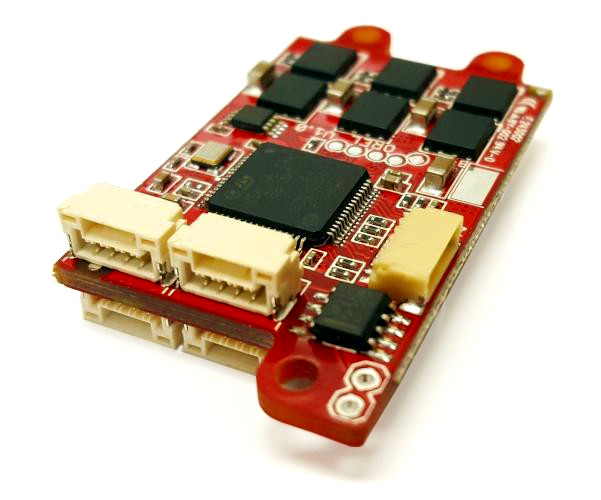
\includegraphics[width=0.45\textwidth]{image}
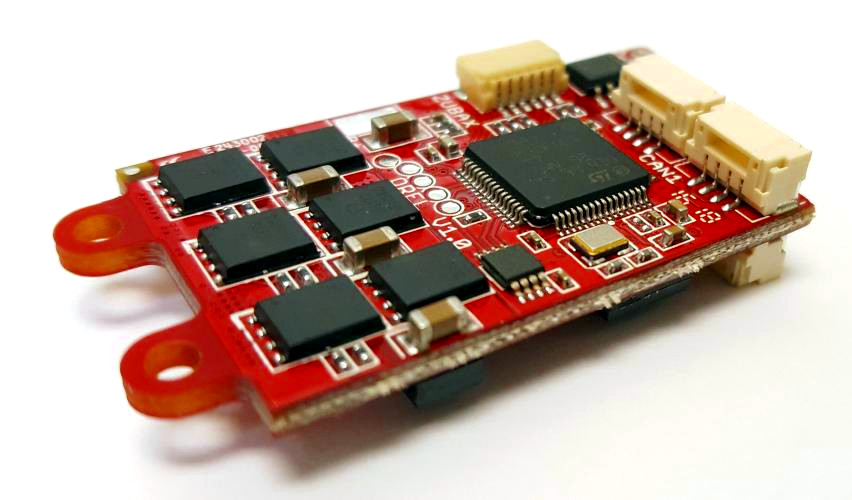
\includegraphics[width=0.45\textwidth]{image2}
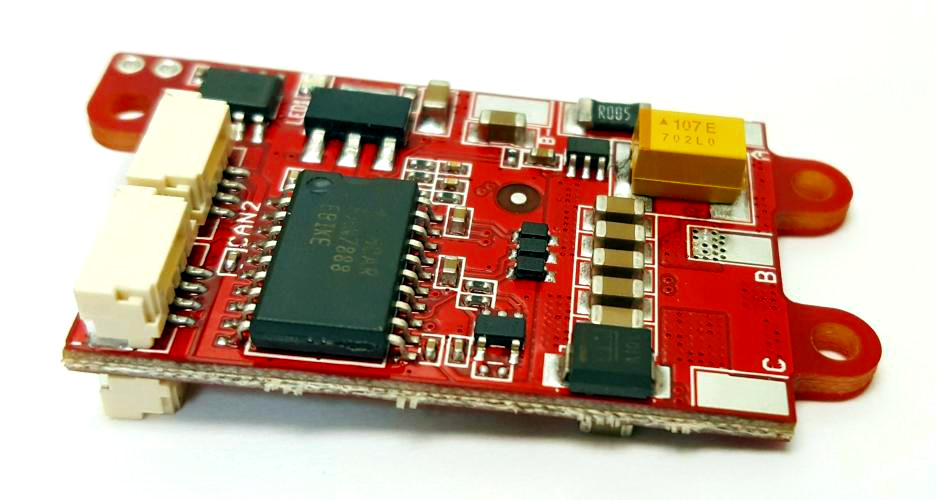
\includegraphics[width=0.45\textwidth]{bottom}

\end{titlepage}

\tableofcontents
\listoffigures
\listoftables

\mainmatter

\chapter{Introduction}

\end{document}
